\chapter{Sous-espaces, projecteurs et mesure comme intrication}

Le théorème de Bell laisse deux questions en suspens. Que reste-t-il de l’intrication lorsqu’un membre d’une paire est perturbé, absorbé ou mesuré ? Et qu’est-ce qui transforme précisément une interaction ordinaire en mesure ? Pour répondre, il faut passer par l’algèbre linéaire élémentaire. Les propriétés sont des sous-espaces, les probabilités sont des valeurs moyennes de projecteurs, et un appareil de mesure est un autre système quantique avec lequel l’objet s’intrique.

\section{Motivation initiale : intrication, localité et mesure}

Supposons qu’un état singulet ait été séparé en deux parties éloignées et que l’une d’elles soit mesurée. La théorie quantique des champs doit-elle décrire un échange virtuel entre les deux ? Rien de détectable ne se produit à l’autre extrémité, et aucun message exploitable n’y parvient. On peut faire tourner localement un spin à l’aide d’un champ magnétique, ce qui modifie la forme détaillée de l’état conjoint, tandis que la quantité d’intrication reste inchangée sous cette opération locale. Nous étudierons plus tard des mesures quantitatives de l’intrication ; pour l’instant, retenons que deux systèmes qui n’interagissent plus ne peuvent pas modifier l’intrication qu’ils partagent par une opération limitée à un seul côté.

\begin{classroomqa}
\lecturetimestamp{00:00:22}
\audiencequestion{Une mesure sur l’un des membres d’un singulet séparé par un intervalle de genre espace exige-t-elle un échange virtuel avec l’autre ?}
\lecturerresponse{Aucun échange détectable ne se produit de l’autre côté. Une opération locale peut faire tourner un facteur et modifier la forme sous laquelle l’état conjoint est écrit, mais elle ne peut pas, à elle seule, transmettre un message ni modifier l’intrication partagée à travers la séparation.}
\end{classroomqa}

Cela oblige à élargir la notion de partenaire. Si l’un des membres d’une paire intriquée tombe dans un trou noir, l’autre ne cesse pas d’être intriqué : il s’intrique avec les degrés de liberté du trou noir, puis, après l’évaporation, avec le rayonnement émis. La même idée ne nécessite aucun trou noir. Plongeons un membre d’une paire intriquée dans une baignoire et laissons-le se mêler violemment à l’eau. Son identité individuelle peut se perdre dans l’état à plusieurs corps, mais la particule éloignée reste intriquée avec la baignoire dans son ensemble, puis finit par l’être avec la vapeur qui s’en échappe.

Il ne s’agit pas seulement d’une histoire de persistance, mais aussi de réversibilité. Si une interaction peut créer de l’intrication, elle peut en principe aussi la défaire. La désintrication est possible, mais seulement si les systèmes entrent de nouveau en contact et interagissent. Tout ce qui peut se produire dans un sens peut se produire dans l’autre.

\begin{classroomqa}
\lecturetimestamp{00:04:45}
\audiencequestion{Si l’on mesure les deux spins d’une paire intriquée, les électrons restent-ils intriqués ? Une seule mesure peut-elle déjà les désintriqu­er ?}
\lecturerresponse{Les mesures peuvent supprimer leur intrication mutuelle, et une seule mesure peut suffire. Pour comprendre ce que cela signifie au lieu de simplement invoquer l’effondrement, nous devons décrire l’observation comme une interaction entre le système et un appareil qui enregistre le résultat.}
\end{classroomqa}

Cette question fixe l’objectif : relier l’observation, l’effondrement du paquet d’ondes et l’intrication. Mais avant de l’aborder, il nous faut une présentation plus nette des sous-espaces et des projecteurs, en n’utilisant pas de notions plus avancées que ne l’exige le raisonnement.

\section{Dimension, dépendance linéaire et bases orthonormées}

Pour l’instant, nous nous en tenons donc aux espaces vectoriels de dimension finie, munis de bras, de kets et d’un produit scalaire. Susskind commence de la manière la plus élémentaire possible. Il ne définit pas la dimension en comptant les composantes d’un vecteur colonne. Il la définit de façon abstraite : la dimension d’un espace vectoriel est le nombre maximal de vecteurs linéairement indépendants que l’on peut y trouver.

Une famille \(\{|v_i\rangle\}\) est donc linéairement indépendante lorsque la relation
\begin{equation}
\sum_i c_i |v_i\rangle = 0
\end{equation}
impose que tous les coefficients \(c_i\) soient nuls. Autrement dit, aucun des vecteurs ne peut s’écrire comme combinaison linéaire des autres.

Il est essentiel de comprendre ici que l’orthogonalité n’est pas la même chose que l’indépendance. Dans un espace de dimension trois, on peut avoir trois vecteurs qui ne sont pas du tout orthogonaux et qui sont pourtant linéairement indépendants. La question est de savoir si l’un d’eux peut être construit à partir des deux autres. En revanche, dans un plan de dimension deux, tout troisième vecteur de ce plan est nécessairement linéairement dépendant des deux premiers.

\begin{figure}[htbp]
\centering
\includegraphics[width=0.56\textwidth]{lecture_06_figure_02.png}
\caption{Trois vecteurs dessinés au tableau. Ce croquis sert à distinguer l’orthogonalité de l’indépendance linéaire, puis à souligner que, dans un plan, un troisième vecteur dépend des deux premiers.}
\lectureframe{00:09:35}
\end{figure}

\begin{figure}[htbp]
\centering
\begin{tikzpicture}[scale=1.2]
\draw[->] (0,0) -- (2.3,0);
\draw[->] (0,0) -- (2.0,2.0);
\draw[->] (0.35,0.95) -- (1.05,1.45);
\fill (0,0) circle (1.2pt);
\end{tikzpicture}
\caption{Reconstitution minimale du croquis au tableau. Le dessin seul ne fixe pas la relation exacte entre les coefficients ; l’idée géométrique est qu’un troisième vecteur d’un plan de dimension deux n’est pas indépendant.}
\end{figure}

C’est ce que montre le croquis. Si l’espace est de dimension deux, le nombre maximal de vecteurs linéairement indépendants est deux. S’il est de dimension trois, ce nombre est trois. Plus généralement, si l’espace est de dimension \(d\), on peut, en présence d’un produit scalaire, trouver \(d\) vecteurs unitaires mutuellement orthogonaux qui engendrent cet espace. Ce sont les vecteurs de base. Susskind précise qu’il ne démontrera pas ce théorème ici. Il veut seulement en retenir la conclusion : dès qu’une telle base existe, tout vecteur de l’espace peut être décomposé suivant ses vecteurs.

\begin{classroomqa}
\lecturetimestamp{00:10:58}
\audiencequestion{Le nombre de degrés de liberté spatiaux est-il le même que la dimension de l’espace des états ?}
\lecturerresponse{Non. Une particule qui se déplace dans une pièce a trois coordonnées spatiales, mais un nombre immense d’états quantiques mutuellement orthogonaux. La dimension de l’espace des configurations et celle de l’espace de Hilbert sont deux notions différentes ; les exemples de dimension finie ne servent ici qu’à exposer clairement le raisonnement.}
\end{classroomqa}

\section{Décomposition sur une base, dyades et résolution de l’identité}

Choisissons maintenant une base orthonormée \(\{|n\rangle\}\), avec \(n=1,\dots,d\). À ce stade, le tableau est particulièrement clair et concis :

\begin{figure}[htbp]
\centering
\includegraphics[width=0.62\textwidth]{lecture_06_figure_03.png}
\caption{Base orthonormée et décomposition d’un état arbitraire.}
\lectureframe{00:14:15}
\end{figure}

On écrit
\begin{align}
\langle m|n\rangle &= \delta_{mn}, \\
|\psi\rangle &= \sum_n a_n |n\rangle.
\end{align}
Ici, \(\delta_{mn}\) est le delta de Kronecker : il vaut \(1\) lorsque \(m=n\) et \(0\) dans le cas contraire.

\paragraph{Démonstration détaillée.} On retrouve les coefficients en projetant sur les vecteurs de base. Multiplions à gauche par \(\langle m|\) :
\begin{align}
\langle m|\psi\rangle
  &= \sum_n a_n \langle m|n\rangle \\
  &= \sum_n a_n \delta_{mn} \\
  &= a_m.
\end{align}
Les coefficients sont donc simplement
\begin{equation}
a_m = \langle m|\psi\rangle.
\end{equation}
Le coefficient est un nombre complexe ordinaire ; on peut donc le placer de part et d’autre du ket sans rien changer.

Si l’on réintroduit cette expression du coefficient dans le développement, on obtient
\begin{equation}
|\psi\rangle = \sum_n |n\rangle \langle n|\psi\rangle.
\end{equation}
Cela suggère que l’objet \(|n\rangle\langle n|\), et plus généralement \(|a\rangle\langle b|\), doit être interprété comme un opérateur. C’est précisément l’étape suivante. Une dyade agit selon
\begin{equation}
\bigl(|a\rangle\langle b|\bigr)|\psi\rangle = \langle b|\psi\rangle\,|a\rangle.
\end{equation}
Le bra extrait un nombre complexe ; le ket fournit la direction qui en résulte. Susskind suit ainsi une voie élémentaire pour passer des vecteurs aux opérateurs.

Interprétons maintenant le développement précédent en termes d’opérateurs. Puisque
\begin{equation}
|\psi\rangle = \left(\sum_n |n\rangle\langle n|\right)|\psi\rangle
\end{equation}
pour tout \(|\psi\rangle\), l’opérateur entre parenthèses doit être l’identité :
\begin{equation}
\sum_n |n\rangle\langle n| = I.
\end{equation}
C’est la résolution de l’identité.

\begin{figure}[htbp]
\centering
\includegraphics[width=0.60\textwidth]{lecture_06_figure_07.png}
\caption{La résolution de l’identité achevée au tableau.}
\lectureframe{00:18:30}
\end{figure}

\begin{classroomqa}
\lecturetimestamp{00:18:39}
\audiencequestion{Les vecteurs de la résolution de l’identité doivent-ils former une base ?}
\lecturerresponse{Oui. La démonstration repose à la fois sur la normalisation et sur l’orthogonalité mutuelle, et la somme doit porter sur une base complète. Une famille arbitraire de vecteurs ne résout pas l’identité.}
\end{classroomqa}

L’opérateur identité est lui-même le projecteur sur l’espace entier. Tout vecteur est vecteur propre de \(I\), et toute valeur propre vaut \(+1\).

\begin{classroomqa}
\lecturetimestamp{00:19:14}
\audiencequestion{La résolution de l’identité signifie-t-elle que tout vecteur a pour valeur propre un ?}
\lecturerresponse{Oui, pour l’opérateur identité. Il est exceptionnel en ce que tout vecteur en est un vecteur propre et que \(I|\psi\rangle=|\psi\rangle\) pour tout état.}
\end{classroomqa}

\section{Les propriétés comme sous-espaces et projecteurs}

Une fois ces outils en place, le cours apporte sa correction conceptuelle centrale. Une propriété telle que \(k=\lambda\) n’est généralement pas un vecteur unique. C’est tout un sous-espace.

Soit \(k\) une observable hermitienne et supposons que
\begin{equation}
k|A\rangle = \lambda |A\rangle, \qquad
k|B\rangle = \lambda |B\rangle,
\end{equation}
avec \(|A\rangle\) et \(|B\rangle\) linéairement indépendants. Alors toute combinaison linéaire a la même valeur propre :
\begin{align}
k\bigl(\alpha|A\rangle+\beta|B\rangle\bigr)
  &= \alpha k|A\rangle + \beta k|B\rangle \\
  &= \alpha \lambda |A\rangle + \beta \lambda |B\rangle \\
  &= \lambda\bigl(\alpha|A\rangle+\beta|B\rangle\bigr).
\end{align}
Le sous-espace propre associé à \(\lambda\) est donc stable par addition et multiplication par un scalaire. C’est un sous-espace vectoriel.

Le premier exemple concret du cours porte sur un système de deux spins. Les états
\begin{equation}
|ud\rangle,\qquad |uu\rangle
\end{equation}
ont des valeurs différentes pour le second spin, mais la même valeur pour le premier : le premier spin est vers le haut dans les deux cas. Ils engendrent donc le sous-espace dans lequel \(\sigma_3=+1\) pour le premier spin.

\begin{figure}[htbp]
\centering
\includegraphics[width=0.46\textwidth]{lecture_06_figure_04.png}
\caption{Deux états de deux spins dont le premier spin est vers le haut.}
\lectureframe{00:23:27}
\end{figure}

Voilà le point à retenir : une propriété n’est pas nécessairement un état unique. C’est tout un ensemble d’états ayant la même valeur propre.

Pour éviter la confusion de notation qui apparaît brièvement au tableau, nous réserverons les majuscules \(A,B,\dots\) aux vecteurs propres particuliers et utiliserons les minuscules \(a,b,\dots\) comme indices de sommation parcourant une base orthonormée du sous-espace propre. Si \(\{|a\rangle\}\) est une telle base du sous-espace \(k=\lambda\), le projecteur sur ce sous-espace est
\begin{equation}
\Pi_{k=\lambda}=\sum_a |a\rangle\langle a|.
\end{equation}
Il s’agit simplement de l’opérateur identité restreint à ce sous-espace. Si \(|\psi\rangle\) appartient déjà à ce sous-espace, le projecteur le laisse inchangé. Si \(|\psi\rangle\) a une composante à l’extérieur, le projecteur élimine la composante orthogonale et ne conserve que celle qui appartient au sous-espace.

\section{Postulat des probabilités, propriétés compatibles et rappel sur Bell}

Dès lors que les propriétés sont réinterprétées comme des sous-espaces, le postulat des probabilités prend sa forme la plus simple. Si \(|\psi\rangle\) est normalisé, la probabilité qu’il possède la propriété \(k=\lambda\) est
\begin{equation}
P(k=\lambda)=\langle\psi|\Pi_{k=\lambda}|\psi\rangle.
\end{equation}

\begin{figure}[htbp]
\centering
\includegraphics[width=0.58\textwidth]{lecture_06_figure_05.png}
\caption{Projecteur sur le sous-espace propre \(k=\lambda\). La disposition au tableau prépare déjà l’étape suivante : placer le projecteur entre \(\langle\psi|\) et \(|\psi\rangle\).}
\lectureframe{00:31:09}
\end{figure}

Insérons l’expression du projecteur en dyades :
\begin{align}
P(k=\lambda)
  &= \left\langle \psi \left| \sum_a |a\rangle\langle a| \right| \psi \right\rangle \\
  &= \sum_a \langle\psi|a\rangle\langle a|\psi\rangle \\
  &= \sum_a |\langle a|\psi\rangle|^2.
\end{align}
C’est exactement l’interprétation proposée dans le cours : la probabilité totale de la propriété est la somme des probabilités de toutes les façons orthogonales dont elle peut se réaliser.

Pour le premier spin orienté vers le haut dans un système de deux spins, le sous-espace pertinent est engendré par \(|uu\rangle\) et \(|ud\rangle\), donc
\begin{equation}
\Pi_{\sigma_3=+1}=|uu\rangle\langle uu|+|ud\rangle\langle ud|.
\end{equation}
Dans la notation abrégée du cours, on écrit aussi
\begin{equation}
\Pi_{\sigma_3=+1}=\frac{1+\sigma_3}{2},
\end{equation}
l’identité sur le second spin étant sous-entendue.

\begin{classroomqa}
\lecturetimestamp{00:33:04}
\audiencequestion{Quelle est la différence entre une observable, une propriété et un projecteur ?}
\lecturerresponse{L’observable est l’opérateur hermitien \(k\). La propriété \(k=\lambda\) est représentée par son sous-espace propre et signifie qu’une mesure de \(k\) donnerait certainement \(\lambda\). Le projecteur \(\Pi_{k=\lambda}\) isole ce sous-espace, et sa valeur moyenne donne la probabilité que la propriété soit présente.}
\end{classroomqa}

\begin{classroomqa}
\lecturetimestamp{00:34:07}
\audiencequestion{Les vecteurs propres dégénérés \(A\) et \(B\) doivent-ils déjà être orthogonaux, et forment-ils une base de tout l’espace ?}
\lecturerresponse{Les vecteurs propres initiaux ne sont pas nécessairement orthogonaux, mais on peut toujours choisir une base orthonormée dans leur sous-espace propre. Elle ne constitue une base que de ce sous-espace ; il faut d’autres directions orthogonales pour engendrer l’espace entier. La projection sur chacun des vecteurs de base du sous-espace, suivie de leur somme, donne le projecteur sur ce sous-espace.}
\end{classroomqa}

\begin{classroomqa}
\lecturetimestamp{00:35:33}
\audiencequestion{Le symbole \(a\) dans \(k|A\rangle=\lambda|A\rangle\) désigne-t-il la même chose que le \(a\) qui intervient dans la somme du projecteur ?}
\lecturerresponse{Non. Le premier désigne un vecteur propre particulier, tandis que l’indice de la somme parcourt tous les vecteurs d’une base orthonormée du sous-espace propre. Une notation distincte évite de confondre un indice fixé avec un indice muet de sommation.}
\end{classroomqa}

\begin{classroomqa}
\lecturetimestamp{00:37:15}
\audiencequestion{Les produits scalaires dans la formule du projecteur sont-ils des probabilités ou des amplitudes de probabilité ?}
\lecturerresponse{Chacun des \(\langle a|\psi\rangle\) est une amplitude. Son produit par son conjugué complexe donne une probabilité ; la somme de ces probabilités sur les différentes réalisations orthogonales de \(k=\lambda\) donne la probabilité totale de la propriété.}
\end{classroomqa}

Le cours examine ensuite comment combiner des propriétés. Supposons que nous ayons deux propriétés compatibles, représentées par les projecteurs commutants \(P_k\) et \(P_\ell\). Dans la formulation du cours, la conjonction est représentée par le produit :
\begin{equation}
\Pi_{k=\lambda\,\wedge\,\ell=\mu}=P_kP_\ell=P_\ell P_k.
\end{equation}
La logique est simple. \(P_k|\psi\rangle\) appartient au sous-espace \(k=\lambda\). Comme les opérateurs commutent, \(P_\ell P_k|\psi\rangle=P_kP_\ell|\psi\rangle\), de sorte que le même vecteur appartient aussi au sous-espace \(\ell=\mu\). Le produit projette donc sur la propriété simultanée. La probabilité correspondante est
\begin{equation}
P(k=\lambda,\ell=\mu)=\langle\psi|P_kP_\ell|\psi\rangle.
\end{equation}

Il vaut la peine d’écrire séparément la première étape de ce raisonnement. Pour tout état,
\begin{equation}
k\bigl(P_k|\psi\rangle\bigr)=\lambda P_k|\psi\rangle,
\end{equation}
donc \(P_k|\psi\rangle\) appartient au sous-espace propre \(k=\lambda\). Si \(P_k\) et \(P_\ell\) commutent, on peut écrire le produit avec l’un ou l’autre des projecteurs à gauche ; le vecteur appartient donc aux deux sous-espaces.

\begin{figure}[htbp]
\centering
\includegraphics[width=0.44\textwidth]{lecture_06_figure_06.png}
\caption{L’état projeté comme vecteur du sous-espace propre.}
\lectureframe{00:41:57}
\end{figure}

\begin{figure}[htbp]
\centering
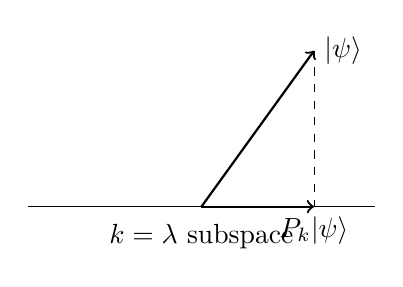
\begin{tikzpicture}[scale=1.1]
\draw (-2,0) -- (2,0);
\draw[->,thick] (0,0) -- (1.3,1.8) node[right] {$|\psi\rangle$};
\draw[dashed] (1.3,1.8) -- (1.3,0);
\draw[->,thick] (0,0) -- (1.3,0) node[below] {$P_k|\psi\rangle$};
\node at (0,-0.35) {$k=\lambda$ subspace};
\end{tikzpicture}
\caption{Projection d’un vecteur arbitraire sur le sous-espace propre \(k=\lambda\).}
\end{figure}

\begin{figure}[htbp]
\centering
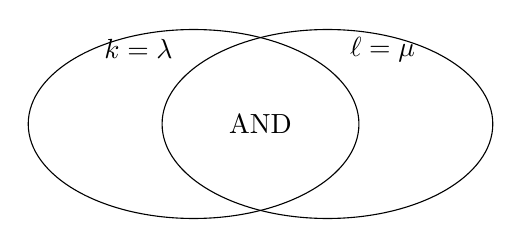
\begin{tikzpicture}[scale=1.0]
\draw (0,0) ellipse (2.1 and 1.2);
\draw (1.7,0) ellipse (2.1 and 1.2);
\node at (-0.7,0.95) {$k=\lambda$};
\node at (2.4,0.95) {$\ell=\mu$};
\node at (0.85,0) {AND};
\end{tikzpicture}
\caption{Reconstitution de la figure des sous-espaces sécants qui sous-tend la conjonction pour des projecteurs commutants.}
\end{figure}

\begin{figure}[htbp]
\centering
\includegraphics[width=0.66\textwidth]{lecture_06_figure_08.png}
\caption{Le raisonnement au tableau montrant que des projecteurs commutants sélectionnent le sous-espace propre simultané.}
\lectureframe{00:45:20}
\end{figure}

\begin{classroomqa}
\lecturetimestamp{00:44:42}
\audiencequestion{La propriété simultanée est-elle identique à l’intersection en logique classique ?}
\lecturerresponse{Oui. Pour des projecteurs commutants, \(P_kP_\ell\) projette sur l’intersection des deux sous-espaces propres. Si cette intersection ne contient que le vecteur nul, aucun état non nul ne possède les deux propriétés.}
\end{classroomqa}

Pour être complet, le projecteur sur le sous-espace de la disjonction compatible est
\begin{equation}
P_{k\lor\ell}=P_k+P_\ell-P_kP_\ell .
\end{equation}
Lorsque les éventualités sont mutuellement exclusives, \(P_kP_\ell=0\), et cette expression se réduit à la somme \(P_k+P_\ell\). Cette soustraction est essentielle dès que les deux sous-espaces se recoupent, car leur intersection ne doit pas être comptée deux fois.

La compatibilité est ensuite reliée à des exemples physiques. Dans un système de deux spins, toute composante \(\sigma_i\) du premier spin commute avec toute composante \(\tau_j\) du second :
\begin{equation}
[\sigma_i,\tau_j]=0.
\end{equation}
En revanche, différentes composantes d’un même spin ne commutent pas :
\begin{equation}
[\sigma_1,\sigma_3]\neq 0.
\end{equation}
C’est pourquoi on peut mesurer une composante de chacun de deux spins séparés, mais pas deux composantes différentes d’un même spin en même temps.

\begin{classroomqa}
\lecturetimestamp{00:46:12}
\audiencequestion{Quels sont des exemples concrets d’observables compatibles ?}
\lecturerresponse{Tout opérateur agissant sur le premier spin commute avec tout opérateur agissant sur le second, car ils agissent sur des facteurs tensoriels différents. Les composantes de position \(x,y,z\) forment également une famille compatible. En revanche, deux composantes différentes d’un même spin, ou la position et son impulsion conjuguée, ne commutent pas.}
\end{classroomqa}

\begin{classroomqa}
\lecturetimestamp{00:47:26}
\audiencequestion{Un sous-système doit-il correspondre à une particule différente ?}
\lecturerresponse{Non. Il s’agit d’un ensemble de degrés de liberté spécifié indépendamment. Des particules distinctes fournissent les facteurs tensoriels les plus simples, mais on peut aussi traiter séparément différents degrés de liberté d’une même particule lorsque la structure de leurs opérateurs le permet.}
\end{classroomqa}

\begin{classroomqa}
\lecturetimestamp{00:48:37}
\audiencequestion{Si tant d’opérateurs portant sur différents sous-systèmes commutent, quel est un exemple simple de paire incompatible ?}
\lecturerresponse{Deux composantes d’un même spin en sont l’exemple classique : \(\sigma_1\) et \(\sigma_3\) ne commutent pas, de sorte qu’aucun appareil ne peut leur attribuer simultanément des valeurs bien définies. La non-nullité du commutateur matriciel en est le critère algébrique.}
\end{classroomqa}

Susskind revient maintenant au théorème de Bell. Il ne reprend pas les calculs de la leçon précédente ; il en reconstruit la logique dans le nouveau langage. L’inégalité classique, sous sa forme probabiliste, est
\begin{equation}
P(A\wedge \neg B)+P(B\wedge \neg C)\ge P(A\wedge \neg C).
\end{equation}
C’est un théorème de la logique classique des ensembles, et non de la mécanique quantique. Dans l’état singulet, les spins sont antiparallèles selon tout axe commun ; on peut donc remplacer une proposition de négation portant sur le premier spin par la proposition positive correspondante portant sur le second. On peut ainsi réécrire l’inégalité en termes de propriétés conjointes d’un système à deux spins.

En omettant les opérateurs identité sur les facteurs qui ne sont pas concernés, les projecteurs de propriétés simples utilisés dans le cours sont
\begin{equation}
\frac{1+\sigma_3}{2},\qquad
\frac{1+\frac{\tau_1+\tau_3}{\sqrt2}}{2},\qquad
\frac{1+\frac{\sigma_1+\sigma_3}{\sqrt2}}{2},\qquad
\frac{1+\tau_1}{2}.
\end{equation}
Les trois projecteurs conjoints pertinents sont donc
\begin{align}
\Pi_1 &= \frac{1+\sigma_3}{2}\,\frac{1+\frac{\tau_1+\tau_3}{\sqrt2}}{2}, \\
\Pi_2 &= \frac{1+\frac{\sigma_1+\sigma_3}{\sqrt2}}{2}\,\frac{1+\tau_1}{2}, \\
\Pi_3 &= \frac{1+\sigma_3}{2}\,\frac{1+\tau_1}{2}.
\end{align}

\begin{figure}[htbp]
\centering
\includegraphics[width=0.68\textwidth]{lecture_06_figure_09.png}
\caption{Les trois choix d’analyseur écrits comme produits de projecteurs portant sur un seul spin.}
\lectureframe{01:01:45}
\end{figure}

Le cours exprime l’état singulet sous la forme familière, non normalisée, du tableau :
\begin{equation}
|\Psi_{\mathrm{singlet}}\rangle \propto |ud\rangle-|du\rangle.
\end{equation}
La proportionnalité suffit ici. Pour le raisonnement, ce qui compte est l’état lui-même et, en particulier, le signe relatif, non la normalisation globale. Le calcul de \(\langle \Pi_1\rangle+\langle \Pi_2\rangle\) et \(\langle \Pi_3\rangle\) dans l’état singulet donne la violation obtenue à la leçon précédente. La conclusion importante est celle que Susskind souligne à l’oral : la mécanique quantique n’est pas la théorie classique des ensembles déguisée.

\begin{classroomqa}
\lecturetimestamp{00:52:31}
\audiencequestion{Si les spins vers le haut et vers le bas sont orthogonaux, le signe moins signifie-t-il qu’un ket est l’opposé de l’autre ?}
\lecturerresponse{Non. \(|u\rangle\) et \(|d\rangle\) sont des vecteurs distincts et orthogonaux. Un signe relatif intervient dans une superposition telle que \(|ud\rangle-|du\rangle\) et peut en modifier les propriétés physiques ; seul un signe global multipliant l’état entier est sans conséquence.}
\end{classroomqa}

\begin{classroomqa}
\lecturetimestamp{00:53:06}
\audiencequestion{L’inégalité de Bell est-elle violée pour tout état quantique et tout choix de propriétés ?}
\lecturerresponse{Non. De nombreux états et de nombreux choix d’axes satisfont une inégalité de Bell donnée. La violation dépend à la fois de l’état et des observables choisies. Modifier les angles intermédiaire et final change la capacité de ce test à mettre en évidence les corrélations non classiques.}
\end{classroomqa}

\begin{classroomqa}
\lecturetimestamp{01:02:47}
\audiencequestion{Que peut-on conclure lorsqu’un état donné viole cette inégalité de Bell, ou se trouve par hasard la satisfaire ?}
\lecturerresponse{Une violation prouve que les statistiques observées ne peuvent pas résulter de la logique classique des ensembles utilisée dans la démonstration. Le fait qu’une inégalité choisie soit satisfaite ne rend pas, à lui seul, l’état classique, car un autre choix de propriétés peut révéler une violation.}
\end{classroomqa}

\section{La localité après Bell}

Le calcul avec les projecteurs n’est pas un simple jeu symbolique. Imaginons que l’on prépare à répétition des paires corrélées dans l’état fondamental singulet, que l’on sépare leurs membres, puis que l’on répartisse l’ensemble préparé de la même façon en trois grands groupes. Le premier groupe est soumis aux réglages \(0^\circ\) et \(45^\circ\), le deuxième aux réglages \(45^\circ\) et \(90^\circ\), et le troisième aux réglages \(0^\circ\) et \(90^\circ\). Les fréquences mesurées dans les trois groupes permettent d’estimer les trois probabilités de l’inégalité.

\begin{classroomqa}
\lecturetimestamp{01:04:30}
\audiencequestion{À quelle configuration expérimentale correspondent les trois probabilités de Bell ?}
\lecturerresponse{Une source produit de nombreuses paires intriquées préparées de façon identique et envoie leurs membres vers des analyseurs séparés. Répartissez les paires en trois ensembles et utilisez pour chacun la paire de directions d’analyse correspondante. Le dénombrement des résultats conjoints permet d’estimer chaque probabilité. Un champ pourrait séparer une particule chargée de son antiparticule ; en pratique, les tests de Bell utilisent souvent des photons.}
\end{classroomqa}

\begin{classroomqa}
\lecturetimestamp{01:08:00}
\audiencequestion{La démonstration classique par les ensembles portait sur une seule population. Comment trois ensembles mesurés séparément peuvent-ils la tester ?}
\lecturerresponse{L’inégalité porte aussi bien sur des probabilités que sur des dénombrements. Si les trois échantillons proviennent de la même procédure de préparation, leurs fréquences relatives estiment les trois distributions de probabilité d’un ensemble commun. L’identité de la préparation est une hypothèse indispensable.}
\end{classroomqa}

Ce rappel du théorème de Bell mène directement à la question physique qui continue de troubler la salle. Si les corrélations sont réelles, pourquoi ne peut-on pas les utiliser pour transmettre un signal ?

\begin{classroomqa}
\lecturetimestamp{01:09:41}
\audiencequestion{Pourquoi ne peut-on pas utiliser les corrélations intriquées pour transmettre un message plus vite que la lumière ?}
\lecturerresponse{Chaque côté observe toujours une suite aléatoire incontrôlable. La corrélation n’apparaît que lorsque l’on compare les deux relevés par un canal classique ordinaire. Un test de Bell décisif organise néanmoins les choix et les détections de sorte qu’aucun signal lumineux ne puisse passer d’un côté à l’autre à temps, excluant ainsi un mécanisme de communication locale susceptible de produire les statistiques conjointes.}
\end{classroomqa}

Si suffisamment de temps s’écoule pour qu’un signal lumineux puisse voyager entre les appareils, une corrélation ne contredit pas à elle seule la relativité ; on a peut-être simplement découvert une influence ordinaire passée inaperçue. L’expérience décisive écarte cette possibilité. Selon la terminologie de Bell, une théorie à variables cachées qui reproduit les corrélations doit être non locale, mais une dépendance non locale n’est pas la même chose qu’un message supraluminique contrôlable.

\begin{classroomqa}
\lecturetimestamp{01:12:18}
\audiencequestion{La conservation du moment cinétique est-elle essentielle à ce raisonnement ?}
\lecturerresponse{Non. Le spin est un modèle commode à deux états, pas un ingrédient indispensable. Toute paire de systèmes à deux niveaux possédant l’état intriqué requis et plusieurs bases de mesure possibles peut présenter la même structure logique.}
\end{classroomqa}

Cette discussion ne clôt pas la leçon ; elle prépare le terrain au prochain changement de perspective. Bell nous a appris que la mécanique quantique n’est pas la logique classique, mais la question suivante est différente. Qu’est-ce qu’une mesure, sur le plan opérationnel et mathématique, et quel rôle joue-t-elle dans l’interférence ?

\section{Expérience des deux fentes à nombre fini d’états, interférence et mesure comme intrication}

Le cours change maintenant de modèle. Susskind passe à l’expérience des deux fentes, mais la simplifie immédiatement en un problème à nombre fini d’états, afin de pouvoir utiliser les mêmes outils d’espace vectoriel sans recourir à tout l’appareil de la mécanique ondulatoire dans un continuum. Il dit même, en substance, qu’il s’agit toujours de l’expérience des deux fentes, simplement réduite à un petit ensemble d’états de base.

Il y a un état source \(|0\rangle\), deux états associés aux fentes \(|1\rangle\) et \(|-1\rangle\), ainsi qu’un ensemble d’états de l’écran \(|n\rangle\). Ces états \(|n\rangle\) sont orthonormés, car des positions distinctes sur l’écran correspondent à des configurations distinctes. Le cours précise qu’à ce stade, il ne s’attache pas à suivre soigneusement la normalisation. L’unitarité est laissée pour plus tard. Pour l’instant, c’est la linéarité qui importe.

\begin{figure}[htbp]
\centering
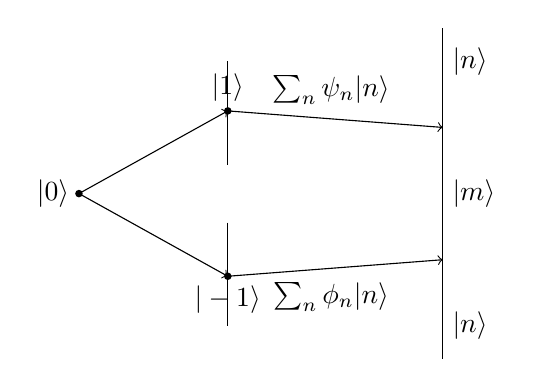
\begin{tikzpicture}[scale=1.05]
\fill (0,0) circle (1.3pt);
\node[left] at (0,0) {$|0\rangle$};

\draw (1.8,1.6) -- (1.8,0.35);
\draw (1.8,-0.35) -- (1.8,-1.6);
\fill (1.8,1) circle (1.3pt);
\fill (1.8,-1) circle (1.3pt);
\node[above] at (1.8,1) {$|1\rangle$};
\node[below] at (1.8,-1) {$|-1\rangle$};

\draw (4.4,2.0) -- (4.4,-2.0);
\node[right] at (4.4,1.6) {$|n\rangle$};
\node[right] at (4.4,0.0) {$|m\rangle$};
\node[right] at (4.4,-1.6) {$|n\rangle$};

\draw[->] (0,0) -- (1.8,1);
\draw[->] (0,0) -- (1.8,-1);
\draw[->] (1.8,1) -- (4.4,0.8);
\draw[->] (1.8,-1) -- (4.4,-0.8);

\node at (3.05,1.25) {$\sum_n \psi_n |n\rangle$};
\node at (3.05,-1.25) {$\sum_n \phi_n |n\rangle$};
\end{tikzpicture}
\caption{Une version à nombre fini d’états de l’expérience des deux fentes : l’état source \(|0\rangle\), les deux états des fentes \(|1\rangle\) et \(|-1\rangle\), et la base de l’écran \(|n\rangle\).}
\end{figure}

\begin{figure}[htbp]
\centering
\includegraphics[width=0.68\textwidth]{lecture_06_figure_10.png}
\caption{Le réseau fini de positions à côté de la règle d’évolution linéaire \(A\to A'\), \(B\to B'\).}
\lectureframe{01:18:00}
\end{figure}

Par symétrie, l’état source évolue vers une superposition des deux états des fentes avec des amplitudes égales :
\begin{equation}
|0\rangle \longrightarrow |1\rangle+|-1\rangle.
\end{equation}
Faisons maintenant évoluer l’état de la fente supérieure selon
\begin{equation}
|1\rangle \longrightarrow \sum_n \psi_n |n\rangle,
\end{equation}
et celui de la fente inférieure selon
\begin{equation}
|-1\rangle \longrightarrow \sum_n \phi_n |n\rangle.
\end{equation}
Les flèches désignent ici l’évolution temporelle, et non l’égalité des états au même instant. Par linéarité,
\begin{equation}
|1\rangle+|-1\rangle \longrightarrow \sum_n (\psi_n+\phi_n)|n\rangle.
\end{equation}
C’est la règle essentielle : les amplitudes s’additionnent avant que l’on calcule les probabilités.

\begin{classroomqa}
\lecturetimestamp{01:21:59}
\audiencequestion{Comment l’état de la fente \(|1\rangle\) peut-il évoluer vers des états eux aussi étiquetés par des entiers \(n\) ? Ces kets correspondent-ils au même lieu et au même instant ?}
\lecturerresponse{Les étiquettes correspondent à des tranches temporelles différentes. \(|1\rangle\) désigne l’électron au niveau de la fente supérieure, tandis que les \(|n\rangle\) de droite désignent ses positions ultérieures possibles sur l’écran. La flèche représente l’évolution temporelle, et non une égalité entre des configurations simultanées.}
\end{classroomqa}

\begin{classroomqa}
\lecturetimestamp{01:25:30}
\audiencequestion{Faut-il normaliser les amplitudes, et ont-elles des unités physiques ?}
\lecturerresponse{Une évolution complète doit préserver la probabilité totale : c’est l’unitarité. Ici, le facteur de normalisation commun est omis, car seule compte l’addition et l’annulation des amplitudes associées aux chemins. On peut rétablir tous les facteurs d’échelle au moment de normaliser l’état.}
\end{classroomqa}

La probabilité d’arrivée sur le site de l’écran \(m\) est donc
\begin{align}
P_m &= |\psi_m+\phi_m|^2 \\
    &= |\psi_m|^2 + |\phi_m|^2 + \psi_m^*\phi_m + \phi_m^*\psi_m.
\end{align}
Les deux premiers termes sont ceux qu’aurait donnés un raisonnement classique. Les deux derniers sont les termes d’interférence.

\begin{figure}[htbp]
\centering
\includegraphics[width=0.68\textwidth]{lecture_06_figure_11.png}
Amplitude sur l’écran et développement en quatre termes de la probabilité correspondante, inscrits au tableau.\caption{}
\lectureframe{01:29:20}
\end{figure}

Au point symétrique de l’écran, que l’on note \(m=0\), la symétrie suggère que \(\psi_0=\phi_0\). On obtient alors
\begin{equation}
P_0 = |\psi_0+\phi_0|^2 = |2\psi_0|^2 = 4|\psi_0|^2.
\end{equation}
Lorsque les deux fentes sont ouvertes, la probabilité en ce point est quatre fois celle obtenue avec une seule fente, et non deux fois. Il s’agit d’interférence constructive.

Insérons maintenant un déphaseur de sorte que \(\phi_0=-\psi_0\). On obtient alors
\begin{equation}
P_0 = |\psi_0-\psi_0|^2 = 0.
\end{equation}
Chaque fente, prise isolément, permet à l’électron d’arriver en ce point, mais les ouvrir toutes les deux peut rendre cette arrivée impossible. Il s’agit d’interférence destructive. Susskind s’attarde explicitement sur le caractère étrange de ce phénomène : selon lui, il est aussi étrange que celui de Bell.

\begin{classroomqa}
\lecturetimestamp{01:33:14}
\audiencequestion{Que se passe-t-il si l’on ne modifie le déphaseur ou le choix de la fente qu’après que l’électron est déjà en vol ? L’autre fente doit-elle avoir le temps de l’apprendre ?}
\lecturerresponse{La réponse dépend de la configuration spatio-temporelle précise et du fait que l’électron rencontre ou non la partie modifiée de l’appareil. En mécanique quantique, l’état évolue selon le dispositif effectivement utilisé ; les probabilités proviennent toujours de l’addition des amplitudes pertinentes. Il faut définir avec précision une expérience à choix retardé avant de pouvoir évaluer les affirmations concernant la localité.}
\end{classroomqa}

Introduisons maintenant l’appareil. Il comporte un système à deux états supplémentaire : un spin initialement dans l’état \(|d\rangle\). Si l’électron passe par la fente supérieure, il fait basculer ce spin dans l’état \(|u\rangle\). S’il passe par la fente inférieure, il le laisse inchangé. L’état initial du système composé est \(|0,d\rangle\), et la première règle d’évolution devient
\begin{equation}
|0,d\rangle \longrightarrow |1,u\rangle + |-1,d\rangle.
\end{equation}
Cette ligne résume à elle seule le sens que prend la mesure dans ce cours. La position de l’électron est désormais intriquée avec l’enregistrement conservé par l’appareil.

\begin{figure}[htbp]
\centering
\includegraphics[width=0.66\textwidth]{lecture_06_figure_12.png}
Le spin du détecteur associe ses enregistrements « haut » et « bas » aux deux alternatives de fente.\caption{}
\lectureframe{01:44:10}
\end{figure}

\begin{classroomqa}
\lecturetimestamp{01:40:20}
\audiencequestion{Faut-il un détecteur à chacune des deux fentes ?}
\lecturerresponse{Un seul détecteur fiable suffit. S’il enregistre le passage par la fente supérieure, un enregistrement inchangé identifie l’alternative inférieure, à condition que chaque électron transmis doive passer par l’une des deux ouvertures. On peut ajouter un second détecteur, mais cela introduit un autre sous-système sans changer le principe.}
\end{classroomqa}

\begin{classroomqa}
\lecturetimestamp{01:40:51}
\audiencequestion{Pourquoi ne pas dire que l’électron passe par les deux fentes ?}
\lecturerresponse{En l’absence d’enregistrement du chemin, l’état est une superposition cohérente et aucun fait rétrospectif ne permet d’établir le chemin emprunté. Lorsqu’une mesure complète du chemin est effectuée, l’appareil enregistre l’une ou l’autre des alternatives à chaque essai. Ce qui subsiste dans les deux alternatives, c’est l’amplitude de l’état, et non deux trajectoires distinctes de l’électron observées séparément.}
\end{classroomqa}

\begin{figure}[htbp]
\centering
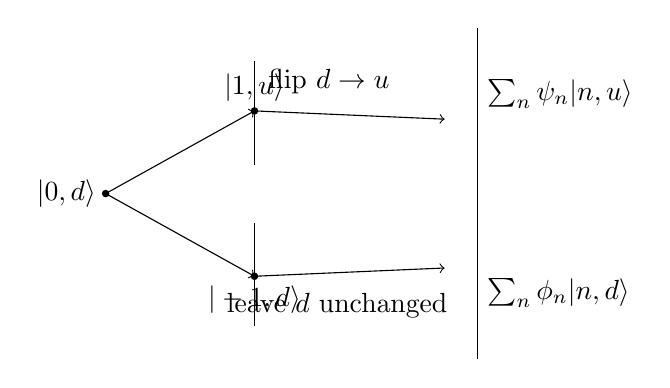
\begin{tikzpicture}[scale=1.05]
\fill (0,0) circle (1.3pt);
\node[left] at (0,0) {$|0,d\rangle$};

\draw (1.8,1.6) -- (1.8,0.35);
\draw (1.8,-0.35) -- (1.8,-1.6);
\fill (1.8,1) circle (1.3pt);
\fill (1.8,-1) circle (1.3pt);
\node[above] at (1.8,1) {$|1,u\rangle$};
\node[below] at (1.8,-1) {$|-1,d\rangle$};

\draw (4.5,2.0) -- (4.5,-2.0);
\node[right] at (4.5,1.2) {$\sum_n \psi_n |n,u\rangle$};
\node[right] at (4.5,-1.2) {$\sum_n \phi_n |n,d\rangle$};

\draw[->] (0,0) -- (1.8,1);
\draw[->] (0,0) -- (1.8,-1);
\draw[->] (1.8,1) -- (4.1,0.9);
\draw[->] (1.8,-1) -- (4.1,-0.9);

\node at (2.7,1.35) {flip \(d\to u\)};
\node at (2.8,-1.35) {leave \(d\) unchanged};
\end{tikzpicture}
La mesure comme intrication avec le spin d’un détecteur. Le chemin supérieur fait basculer le spin de l’appareil ; le chemin inférieur le laisse inchangé.\caption{}
\end{figure}

Supposons, comme le fait le cours, que rien d’autre n’arrive au spin pendant le trajet jusqu’à l’écran. Alors
\begin{align}
|1,u\rangle &\longrightarrow \sum_n \psi_n |n,u\rangle, \\
|-1,d\rangle &\longrightarrow \sum_n \phi_n |n,d\rangle.
\end{align}
L’état final lorsque les deux fentes sont ouvertes est donc
\begin{equation}
|\Psi_{\mathrm{final}}\rangle
  = \sum_n \psi_n |n,u\rangle + \sum_n \phi_n |n,d\rangle.
\end{equation}
Il ne s’agit pas d’une superposition d’états de l’électron seul, mais d’un état intriqué de l’électron et de l’appareil.

\begin{figure}[htbp]
\centering
\includegraphics[width=0.68\textwidth]{lecture_06_figure_13.png}
Les amplitudes associées aux deux chemins arrivent à l’écran avec des enregistrements orthogonaux de l’appareil.\caption{}
\lectureframe{01:47:35}
\end{figure}

La méthode la plus directe pour calculer la probabilité d’arrivée sur le site \(m\) consiste à utiliser le projecteur sur ce site dans le sous-système de l’électron :
\begin{equation}
\Pi_m = |m\rangle\langle m|\otimes I_{\mathrm{spin}}.
\end{equation}
L’application de \(\Pi_m\) à l’état final donne
\begin{equation}
\Pi_m |\Psi_{\mathrm{final}}\rangle
= |m\rangle\bigl(\psi_m|u\rangle+\phi_m|d\rangle\bigr).
\end{equation}
La probabilité d’arrivée en \(m\) est donc
\begin{align}
P_m
  &= \langle \Psi_{\mathrm{final}}|\Pi_m|\Psi_{\mathrm{final}}\rangle \\
  &= \bigl(\psi_m^*\langle u|+\phi_m^*\langle d|\bigr)
     \bigl(\psi_m|u\rangle+\phi_m|d\rangle\bigr) \\
  &= |\psi_m|^2 + |\phi_m|^2
     + \psi_m^*\phi_m\langle u|d\rangle
     + \phi_m^*\psi_m\langle d|u\rangle.
\end{align}
Or, les états correspondant aux enregistrements sont orthogonaux :
\begin{equation}
\langle u|d\rangle=0.
\end{equation}
Les termes croisés s’annulent donc :
\begin{equation}
P_m = |\psi_m|^2 + |\phi_m|^2.
\end{equation}
C’est le résultat mathématique clé du cours. Dès que l’information sur le chemin est enregistrée, l’interférence disparaît et les probabilités s’additionnent comme en physique classique.

\begin{classroomqa}
\lecturetimestamp{01:49:09}
\audiencequestion{Quelle différence y a-t-il entre la superposition \(|1\rangle+|-1\rangle\) et l’état \(|1,u\rangle+|-1,d\rangle\) ?}
\lecturerresponse{La première concerne un seul système dans une combinaison linéaire de deux positions ; il n’y a aucun autre système avec lequel il pourrait être intriqué. Le second concerne deux systèmes et associe le chemin au spin du détecteur. La lecture du spin fournit alors des informations sur le chemin.}
\end{classroomqa}

\section{Enregistrements environnementaux et mesure partielle}

Un détecteur conçu à cet effet n’est pas le seul dispositif susceptible de conserver une trace. Un atome près d’une fente, un gaz résiduel, une surface thermique ou tout autre degré de liberté peut se corréler au chemin. Si ses états finaux sont \(|E_1\rangle\) et \(|E_2\rangle\), l’état associé aux chemins prend la forme
\begin{equation}
|\Psi\rangle
=\sum_n\left(\psi_n|n\rangle|E_1\rangle
+\phi_n|n\rangle|E_2\rangle\right).
\end{equation}
Les termes d’interférence sont maintenant multipliés par le recouvrement \(\langle E_1|E_2\rangle\). Des enregistrements orthogonaux rendent les chemins parfaitement distinguables et suppriment complètement l’interférence. Des enregistrements identiques donnent \(\langle E_1|E_2\rangle=1\) et préservent l’interférence. Un recouvrement intermédiaire produit une visibilité partielle.

\begin{figure}[htbp]
\centering
\includegraphics[width=0.68\textwidth]{lecture_06_figure_14.png}
Des paquets d’onde environnementaux qui se recouvrent ou sont séparés illustrent des enregistrements partiels ou complets du chemin.\caption{}
\lectureframe{01:53:40}
\end{figure}

\begin{classroomqa}
\lecturetimestamp{01:50:48}
\audiencequestion{Un atome ordinaire près de la fente s’intrique-t-il avec l’électron qui passe, même si personne ne l’observe délibérément ?}
\lecturerresponse{Oui. Ce qui compte, ce n’est pas la connaissance, mais la corrélation physique. Si l’atome ou le gaz environnant est suffisamment perturbé pour que son état ultérieur permette de distinguer le chemin, il enregistre l’information sur celui-ci et atténue l’interférence. C’est pourquoi ces expériences nécessitent un isolement, de basses températures et souvent des particules qui interagissent peu, comme les photons.}
\end{classroomqa}

Le refroidissement rapproche les degrés de liberté environnementaux de leur état fondamental et réduit les enregistrements accidentels. La présence d’un écart d’énergie est également utile : si la particule incidente ne peut fournir l’énergie minimale d’excitation, l’environnement peut être incapable de conserver une information sur le chemin. À l’inverse, les particules chargées peuvent perturber la matière voisine par leur champ électrique, ce qui rend particulièrement exigeantes les expériences d’interférence avec des électrons.

\begin{classroomqa}
\lecturetimestamp{01:54:49}
\audiencequestion{Peut-on réellement obtenir une figure d’interférence avec des électrons individuels ?}
\lecturerresponse{Chaque électron ne produit qu’un impact localisé. Faisons passer les particules une à une, en les espaçant suffisamment pour qu’elles ne puissent pas interagir, puis répétons l’expérience de nombreuses fois. La distribution des fréquences ainsi accumulées fait apparaître la figure d’interférence ; un seul événement ne produit qu’un point.}
\end{classroomqa}

\begin{classroomqa}
\lecturetimestamp{01:55:59}
\audiencequestion{La mesure détruit-elle l’intrication ou la crée-t-elle ?}
\lecturerresponse{L’interaction qui détermine le chemin crée une intrication entre le système et l’appareil, et cette intrication détruit l’interférence entre les alternatives. Une mesure ultérieure peut corréler l’appareil à un autre système et conditionner l’état restant ; il faut donc toujours préciser quels sont les deux sous-systèmes concernés et de quelle interférence il est question.}
\end{classroomqa}

\begin{classroomqa}
\lecturetimestamp{01:57:44}
\audiencequestion{Peut-on affaiblir l’interaction pour que l’appareil n’obtienne qu’une information partielle sur le chemin ?}
\lecturerresponse{Oui. Une interaction faible peut faire basculer le détecteur avec une amplitude donnée, laissant des états d’enregistrement non orthogonaux. Les chemins ne sont alors que partiellement distinguables et l’interférence n’est que partiellement réduite. Une mesure plus forte signifie une meilleure distinction entre les chemins, une intrication plus forte avec l’enregistrement et une visibilité plus faible des franges.}
\end{classroomqa}

L’effondrement pertinent ici est donc un phénomène concret : il correspond à la disparition des termes croisés lorsque l’information sur le chemin est déposée dans un autre système. Sans enregistrement, les amplitudes s’additionnent. Avec des enregistrements parfaitement distinguables, leurs produits scalaires s’annulent et les probabilités s’additionnent. Entre ces deux cas limites, l’intensité de la mesure et la visibilité des franges varient continûment.
